\section{Introduction}\label{introduction}

\begin{frame}{Motivation}

\begin{itemize}
\item
  Renewable energy scenarios are important in many fields in Power
  Systems:

  \begin{enumerate}
  \def\labelenumi{\roman{enumi})}
  \tightlist
  \item
    Energy trading;
  \item
    unit commitment;
  \item
    grid expansion planning;
  \item
    investment decisions
  \end{enumerate}
\item
  In stochastic optimization problems, a set of scenarios is a needed
  input.
\item
  Robust optimization requires bounds for probable values.
\end{itemize}

\textbf{Change in paradigm: from predicting the conditional mean to
predicting the conditional distribution}

\end{frame}

\begin{frame}{Probability Forecasting Approaches}

\begin{itemize}
\tightlist
\item
  \emph{Parametric Models}

  \begin{itemize}
  \tightlist
  \item
    Assume a distributional shape
  \item
    Low computational costs
  \item
    Faster convergence
  \item
    \emph{Examples: Arima-GARCH, GAS}
  \end{itemize}
\item
  \emph{Nonparametric Models}

  \begin{itemize}
  \tightlist
  \item
    Don't require a distribution to be specified
  \item
    High computational cost
  \item
    Needs more data to produce a good approximation
  \item
    \emph{Examples: Quantile Regression (Koenker and Bassett Jr (1978)),
    Kernel Density Estimation (Gallego-Castillo et al. (2016)),
    Artificial Intelligence (Wan et al. (2017))}
  \end{itemize}
\end{itemize}

\end{frame}

\begin{frame}{Wind Power Time Series - Icaraizinho}

\begin{figure}
    \centering
    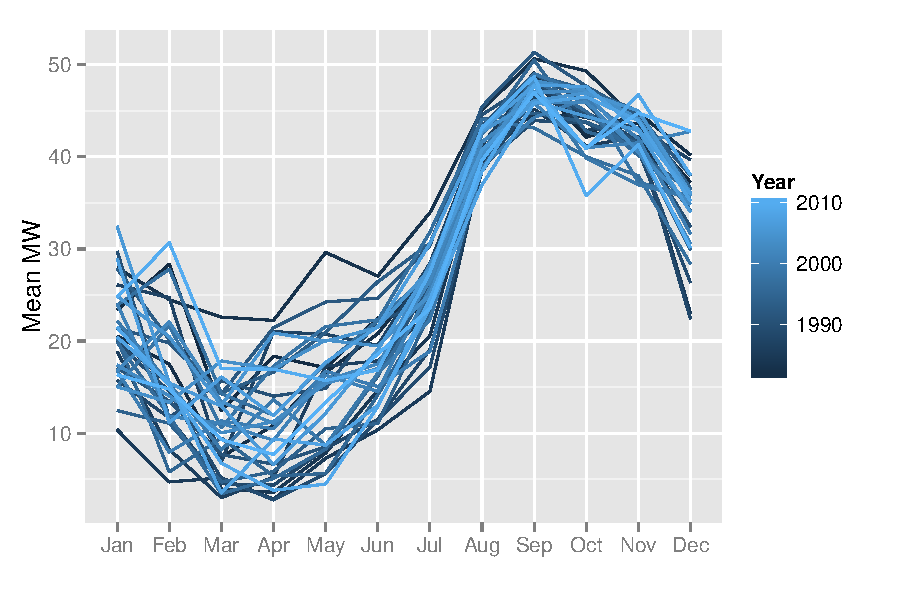
\includegraphics[width=0.9\linewidth]{Imagens/icaraizinho-mensal}
\end{figure}

\end{frame}

\begin{frame}{The nongaussianity of Wind Power}

\begin{figure}
    \centering
    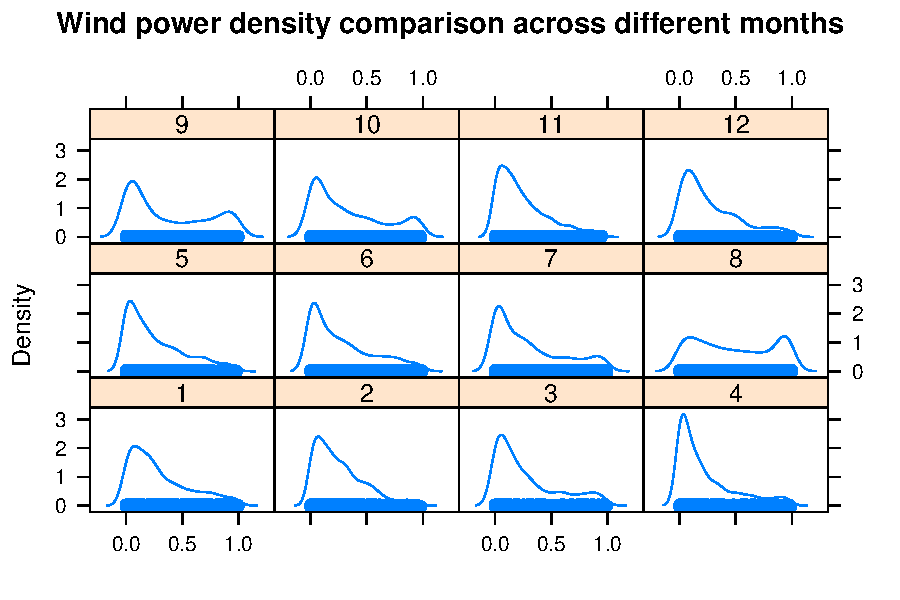
\includegraphics[width=0.9\linewidth]{Imagens/density}
\end{figure}

\end{frame}

\begin{frame}{The nongaussianity of Wind Power}

\begin{itemize}
\tightlist
\item
  Renewables, such as wind and solar power have reportedly nongaussian
  behaviour
\item
  Convenience of using a nonparametric approach, which doesn't rely on
  assuming a distribution
\item
  Quantile regression is the chosen technique available to model this
  time series dynamics, by estimating a thin grid of
  \(\alpha\)-quantiles at once and forming a data-driven conditional
  distribution
\end{itemize}

\end{frame}

\section{Quantile Regression}\label{quantile-regression}

\begin{frame}{Definition of the Conditional Quantile}

Let the \(\alpha\)-conditional quantile function of \(Y\) for a given
value \(x\) of the \(d\)-dimensional random variable \(X\), i.e.,
\(Q_{Y|X}:[0,1] \times \mathbb{R}^d \rightarrow \mathbb{R}\), can be
defined as:
\[Q_{Y|X}(\alpha,x) = F_{Y|X=x}^{-1}(\alpha) = \inf\{y: F_{Y|X=x}(y) \geq \alpha\}.\]

\end{frame}

\begin{frame}{Conditional Quantile from a sample}

Let a dataset be composed from \(\{y_t,x_t \}_{t \in T}\) and let
\(\rho\) be the check function

\begin{equation}\label{eq:check-function}
\rho_{\alpha}(x)=\begin{cases}
\alpha x & \text{if }x\geq0\\
(1-\alpha)x & \text{if }x<0
\end{cases},
\end{equation}

The sample quantile function for a given probability \(\alpha\) is then
based on a finite number of observations and is the solution to
minimizing the loss function \(L(\cdot)\):

\begin{eqnarray}
\hat{Q}_{Y|X}(\alpha,\cdot)\quad\in\quad  \underset{q(\cdot)\in\mathcal{Q}}{\text{arg min}}\, L_\alpha(q) = \sum_{t\in T}\rho_{\alpha}(y_{t}-q(x_t)).\label{eq:optim-lqr1}, 
\end{eqnarray}

where \(\mathcal{Q}\) is a space of functions. In this paper, we use
\(\mathcal{Q}\) as an \textbf{affine functions space}.

\end{frame}

\begin{frame}{Conditional Quantile from a sample}

\begin{itemize}
\tightlist
\item
  For a single quantile, the problem (\ref{eq:optim-lqr1}) can be solved
  by the following Linear Programming problem: \[
  \begin{array}{lll}
   \underset{\beta_0, \beta,\varepsilon_{t}^{+}, \varepsilon_{t}^{-}}{\text{min}} & \sum_{t \in T} \left(\alpha \varepsilon_{t}^{+}+(1-\alpha)\varepsilon_{t}^{-}\right) & \\
  \mbox{s.t. } & \varepsilon_{t}^{+}-\varepsilon_{t}^{-}=y_{t} - \beta_{0} - \beta^T x_{t}, & \qquad\forall t \in T,\\
  & \varepsilon_t^+,\varepsilon_t^- \geq 0, & \qquad \forall t \in T.
  \end{array}
  \]
\item
  The output are the coefficients \(\beta_0\) and \(\beta\) (which is
  the same dimension as \(x_t\)), that describe describes the quantile
  function as an affine function.
\end{itemize}

\end{frame}

\begin{frame}{The non-crossing issue}

\begin{figure}
  \centering
  \begin{minipage}[t]{\linewidth}
    \centering
    \begin{minipage}[t]{0.45\linewidth}
      \centering     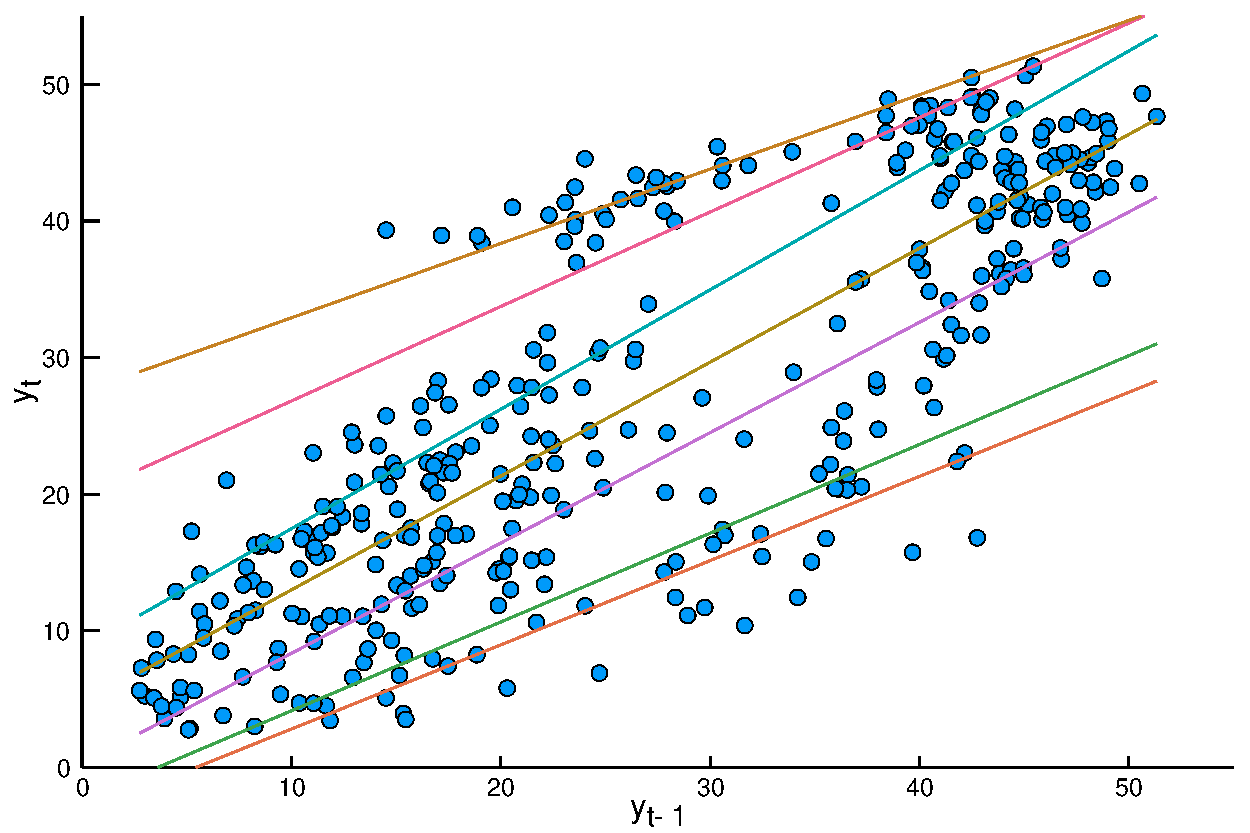
\includegraphics[width=\textwidth]{Imagens/icaraizinho-quantile-linear-scatter}
    \end{minipage}
    \begin{minipage}[t]{0.45\linewidth}
      \centering     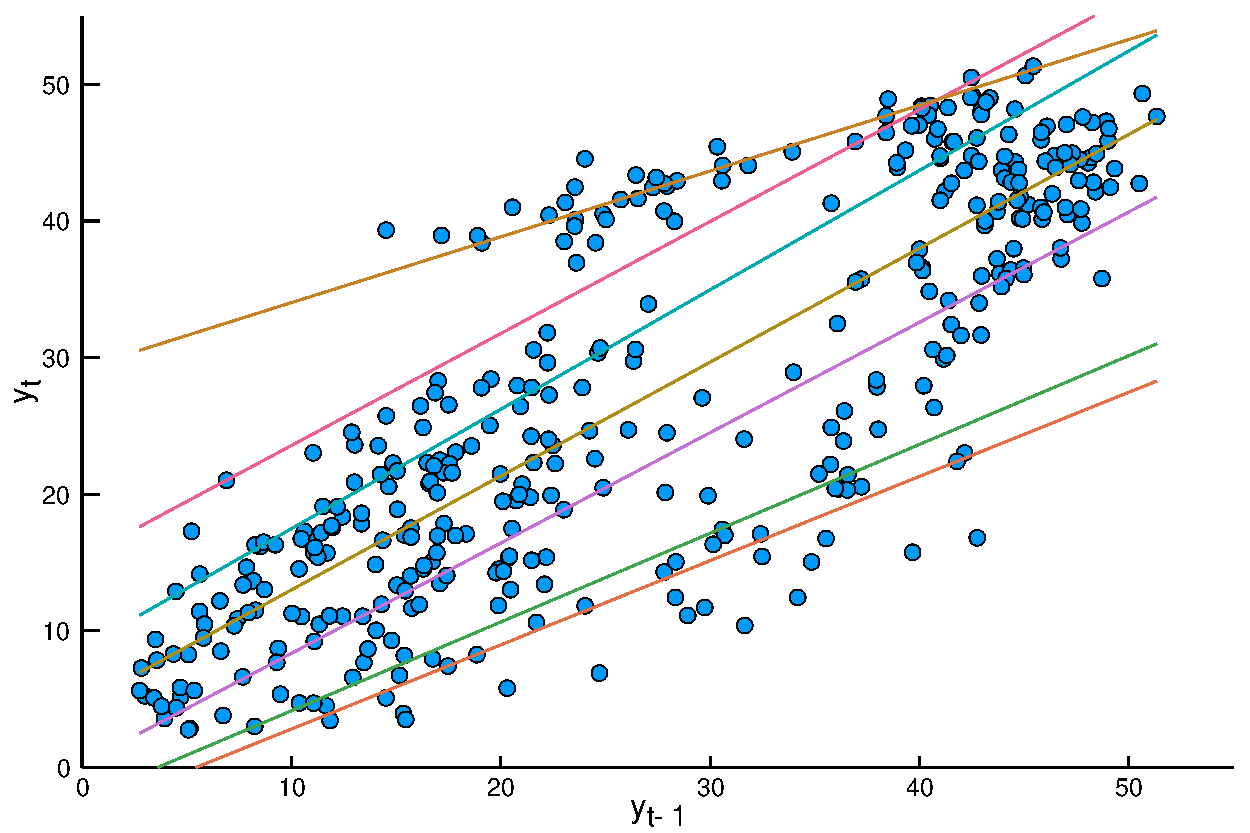
\includegraphics[width=\textwidth]{Imagens/icaraizinho-quantile-linear-scatter-crossing}
    \end{minipage}
  \end{minipage}
  \caption{Estimated quantile functions, for different values of $y_{t-1}$. On the left using a linear model and using a nonparametric approach on the right.}
  \label{fig:quantiles-vs-xt}
\end{figure}

\end{frame}

\begin{frame}{Notation}

\small

\begin{longtable}[]{@{}ll@{}}
\toprule
\begin{minipage}[b]{0.14\columnwidth}\raggedright\strut
Expression\strut
\end{minipage} & \begin{minipage}[b]{0.80\columnwidth}\raggedright\strut
Meaning\strut
\end{minipage}\tabularnewline
\midrule
\endhead
\begin{minipage}[t]{0.14\columnwidth}\raggedright\strut
\(Q_{Y \mid X}(\alpha,x)\)\strut
\end{minipage} & \begin{minipage}[t]{0.80\columnwidth}\raggedright\strut
The conditional quantile function\strut
\end{minipage}\tabularnewline
\begin{minipage}[t]{0.14\columnwidth}\raggedright\strut
\(y_t\)\strut
\end{minipage} & \begin{minipage}[t]{0.80\columnwidth}\raggedright\strut
the time series we are modelling\strut
\end{minipage}\tabularnewline
\begin{minipage}[t]{0.14\columnwidth}\raggedright\strut
\(x_t\)\strut
\end{minipage} & \begin{minipage}[t]{0.80\columnwidth}\raggedright\strut
explanatory variables of \(y_t\) in \(t\)\strut
\end{minipage}\tabularnewline
\begin{minipage}[t]{0.14\columnwidth}\raggedright\strut
\(T\)\strut
\end{minipage} & \begin{minipage}[t]{0.80\columnwidth}\raggedright\strut
the set containing all observations indexes\strut
\end{minipage}\tabularnewline
\begin{minipage}[t]{0.14\columnwidth}\raggedright\strut
\(J\)\strut
\end{minipage} & \begin{minipage}[t]{0.80\columnwidth}\raggedright\strut
the set containing all quantile indexes\strut
\end{minipage}\tabularnewline
\begin{minipage}[t]{0.14\columnwidth}\raggedright\strut
\(J_{(-1)}\)\strut
\end{minipage} & \begin{minipage}[t]{0.80\columnwidth}\raggedright\strut
the set \(J\backslash \{1\}\)\strut
\end{minipage}\tabularnewline
\begin{minipage}[t]{0.14\columnwidth}\raggedright\strut
\(\alpha_j\)\strut
\end{minipage} & \begin{minipage}[t]{0.80\columnwidth}\raggedright\strut
a probability, might be indexed by \(j\)\strut
\end{minipage}\tabularnewline
\begin{minipage}[t]{0.14\columnwidth}\raggedright\strut
\(A\)\strut
\end{minipage} & \begin{minipage}[t]{0.80\columnwidth}\raggedright\strut
the set of probabilities \(\{\alpha_j \mid j \in J\}\)\strut
\end{minipage}\tabularnewline
\begin{minipage}[t]{0.14\columnwidth}\raggedright\strut
\(K\)\strut
\end{minipage} & \begin{minipage}[t]{0.80\columnwidth}\raggedright\strut
Maximum number of covariates on MILP regularization\strut
\end{minipage}\tabularnewline
\begin{minipage}[t]{0.14\columnwidth}\raggedright\strut
\(\lambda\)\strut
\end{minipage} & \begin{minipage}[t]{0.80\columnwidth}\raggedright\strut
The Lasso penalization on the coefficients \(\ell_1\)-norm\strut
\end{minipage}\tabularnewline
\begin{minipage}[t]{0.14\columnwidth}\raggedright\strut
\(\gamma\)\strut
\end{minipage} & \begin{minipage}[t]{0.80\columnwidth}\raggedright\strut
The penalization on the coefficients second-derivative with respect of
the quantiles\strut
\end{minipage}\tabularnewline
\bottomrule
\end{longtable}

\end{frame}

\begin{frame}{Conditional Quantile as a Linear Programming Problem}

\[
\min_{\beta_{0j},\beta_j,\varepsilon_{tj}^{+}, \varepsilon_{tj}^{-}} \, \sum_{j \in J} \sum_{t \in T}\left(\alpha_j \varepsilon_{t j}^{+}+(1-\alpha_j)\varepsilon_{t j}^{-}\right)
\] \[
\begin{array}{lr}
\text{s.t.} &\\
\varepsilon_{t j}^{+}-\varepsilon_{t j}^{-}=y_{t} - \beta_{0j} - \beta_{j}^T x_{t}, & \forall t \in T, \forall j \in J, \\
\varepsilon_{tj}^+,\varepsilon_{tj}^- \geq 0, & \forall t \in T,\forall j \in J,\\
\beta_{0,j-1} + \beta_{j-1}^T x_{t} \leq \beta_{0j} + \beta_{j}^T x_{t},
& \forall t \in T, \forall j \in J_{(-1)},
\end{array}
\]

We apply QR to estimate the conditional distribution
\(\hat{Q}_{Y_{t+h}|X_{t+h},Y_t, Y_{t-1}, \dots} (\alpha,\cdot)\) for a
\(k\)-step ahead forecast of time serie \(\{y_t\}\), where \(X_{t+h}\)
is a vector of exogenous variables at the time we want to forecast.

\end{frame}

\section{Regularization}\label{regularization}

\begin{frame}{Best Subset selection via MILP}

\begin{itemize}
\item
  Mixed Integer Linear Programming (MILP) models allow only \(K\)
  variables to be used for each \(\alpha\)-quantile. This means that
  only \(K\) coefficients \(\beta_{pj}\) may have nonzero values, for
  each \(\alpha\)-quantile. It must be guaranteed by constraints on the
  optimization problem.
\item
  We present three forms of regularization using MILP
\end{itemize}

\end{frame}

\begin{frame}{MILP - One model for each \(\alpha\)-quantile}

\[
\begin{array}{lll}
 \underset{\beta_{0j},\beta_j,z_{p j} \varepsilon_{t j}^{+},\varepsilon_{t j}^{-}}{\text{min}} & \sum_{j \in J} \sum_{t\in T}\left(\alpha_j\varepsilon_{t j}^{+}+(1-\alpha_j)\varepsilon_{t j}^{-}\right)  & \\
\mbox{s.t } & \varepsilon_{t j}^{+}-\varepsilon_{t j}^{-}=y_{t}-\beta_{0 j}-\sum_{p=1}^{P}\beta_{p j}x_{t,p},& \forall t \in T ,\forall j \in J, \\
& \varepsilon_{t j}^{+},\varepsilon_{t j}^{-}\geq0,&\forall t \in T ,\forall j \in J, \\
& - M z_{p j} \leq \beta_{p j} \leq M z_{p j},& \forall j \in J, \forall p\in P, \\
& \sum_{p=1}^P z_{p j} \leq K, &  \forall j \in J, \\
& z_{p j} \in \{0,1\},& \forall j \in J, \forall p\in P,\\
& \beta_{0,j-1} + \beta_{j-1}^T x_{t} \leq \beta_{0,j} + \beta_{j}^T x_{t}, & \forall t \in T, \forall j \in J_{(-1)},
\end{array}
\]

\end{frame}

\begin{frame}{MILP - Defining groups for \(\alpha\)-quantiles}

\[
\begin{array}{lll}
 \underset{\beta_{0j},\beta_j,z_{p j}, \varepsilon_{t j}^{+},\varepsilon_{t j}^{-}}{\text{min}} & \sum_{j \in J} \sum_{t\in T}\left(\alpha_j\varepsilon_{t j}^{+}+(1-\alpha_j)\varepsilon_{t j}^{-}\right)  & \\
\mbox{s.t } & \varepsilon_{t j}^{+}-\varepsilon_{t j}^{-}=y_{t}-\beta_{0 j}-\beta_{j}^T x_{t,p},& \forall t \in T ,\forall j \in J, \\
& \varepsilon_{t j}^{+},\varepsilon_{t j}^{-}\geq0,&\forall t \in T ,\forall j \in J, \\
& - M z_{p j g} \leq \beta_{p j} \leq M z_{p j g},& \forall j \in J, \forall p\in P,  \\
& & \quad \forall g \in G \\
&z_{p j g} := 2 - ( 1-z_{pg}) - I_{gj}& \\
& \sum_{p=1}^P z_{p g} \leq K, &  \forall j \in J, \\
& \beta_{0,j-1} + \beta_{j-1}^T x_{t} \leq \beta_{0j} + \beta_{j}^T x_{t}, & \forall t \in T, \forall j \in J_{(-1)},\\
& I_{gj}, z_{pg} \in \{0,1\},& \forall p \in P,\forall g \in G, \\
& z_{p g} \in \{0,1\},& \forall j \in J, \forall p\in P,\\
\end{array}
\]

\end{frame}

\begin{frame}{MILP - Penalization of derivative}

\tiny

\begin{eqnarray}
 \underset{\beta_{0j},\beta_j,z_{p j} \varepsilon_{t j}^{+},\varepsilon_{t j}^{-}}{\text{min}} & \sum_{j \in J} \sum_{t\in T}\left(\alpha_k \varepsilon_{t j}^{+}+(1-\alpha_k)\varepsilon_{t\alpha}^{-}\right) + \gamma \sum_{j \in J'} D2_{p\alpha} \span \\
\mbox{s.t } & \varepsilon_{t j}^{+}-\varepsilon_{t j}^{-}=y_{t}-\beta_{0 j}-\sum_{p=1}^{P}\beta_{p j}x_{t,p},& \forall t \in T ,\forall j \in J, \\
& \varepsilon_{t j}^{+},\varepsilon_{t j}^{-}\geq0,&\forall t \in T ,\forall j \in J, \label{eq:mip2}\\
& - M z_{p j} \leq \beta_{p j} \leq M z_{p j},& \forall j \in J, \forall p\in P, \label{eq:mip3}\\
& \sum_{p=1}^P z_{p j} \leq K, & \qquad \forall j \in J, \label{eq:mip4}\\
& z_{p j} \in \{0,1\},& \forall j \in J, \forall p\in P, \label{eq:mip5}\\
& \tilde{D}_{pj}^{2}=\frac{\left(\frac{\beta_{p,j+1}-\beta_{pj}}{\alpha_{j+1}-\alpha_{j}}\right)-\left(\frac{\beta_{p,j}-\beta_{p,j-1}}{\alpha_{J}-\alpha_{j-1}}\right)}{\alpha_{j+1}-2\alpha_{j}+\alpha_{j-1}} \span\\
& D2_{pj} >  \tilde D_{pj}^{2} &  \forall j \in J_{(-1)}, \forall p\in P, \\
& D2_{pj} >  - \tilde D_{pj}^{2} &  \forall j \in J_{(-1)}, \forall p\in P,\\
& \beta_{0,j-1} + \beta_{j-1}^T x_{t} \leq \beta_{0j} + \beta_{j}^T x_{t}, & \forall t \in T, \forall j \in J_{(-1)},
\end{eqnarray}

\end{frame}

\begin{frame}{Variable Selection via LASSO}

\begin{itemize}
\tightlist
\item
  Another way of doing regularization is including the coefficients
  \(\ell_1\)-norm on the objective function
\item
  In this method, coefficients are shrunk towards zero by changing a
  continuous parameter \(\lambda\), which penalizes the size of the
  \(\ell_1\)-norm.\\
\item
  When the value of \(\lambda\) gets bigger, fewer variables are
  selected to be used.
\item
  The optimization problem for a single quantile is presented below: \[
  \underset{\beta_{0},\beta}{\text{min}} \sum_{t \in T}\alpha|y_{t}-q(x_t)|^{+}+ \sum_{t \in T}(1-\alpha)|y_{t}-q(x_t)|^{-}+\lambda\|\beta\|_{1},
  \]
\end{itemize}

\[
q(x_t)=\beta_{0}-\sum_{p=1}^{P}\beta_{p}x_{t,p}.
\]

\end{frame}

\begin{frame}{Variable Selection via LASSO}

\begin{itemize}
\tightlist
\item
  At first, we select variables using LASSO
\end{itemize}

\tiny

\begin{eqnarray}
\underset{\beta_{0},\beta,\varepsilon_{t j}^{+},\varepsilon_{t j}^{-}}{\text{arg min}} & \sum_{j \in J} \sum_{t \in T}\left(\alpha_j \varepsilon_{t j}^{+}+(1-\alpha_j)\varepsilon_{t j}^{-}\right)+\lambda\sum_{p=1}^{P}\mbox{\ensuremath{\xi}}_{p j} + \gamma \sum_{j \in J'} D2_{pj} \span \label{eq:obj-lasso} \\
\mbox{s.t. } & \varepsilon_{t j}^{+}-\varepsilon_{t j}^{-}= y_{t}-\beta_{0 j}-\sum_{p=1}^{P}\beta_{p j}\tilde x_{t,p},&\forall t\in T, \forall j \in J, \\
& \varepsilon_{t j}^{+},\varepsilon_{t j}^{-}\geq0,&\forall t \in T, \forall j \in J,\\
& \xi_{p\alpha}\geq\beta_{p j},&\forall p\in P, \forall j \in J,  \label{l1-qar-3}
\\
& \tilde{D}_{pj}^{2}=\frac{\left(\frac{\beta_{p,j+1}-\beta_{pj}}{\alpha_{j+1}-\alpha_{j}}\right)-\left(\frac{\beta_{p,j}-\beta_{p,j-1}}{\alpha_{J}-\alpha_{j-1}}\right)}{\alpha_{j+1}-2\alpha_{j}+\alpha_{j-1}} \span\\
& D2_{pj} >  \tilde D_{pj}^{2} &  \forall j \in J_{(-1)}, \forall p\in P, \\
& D2_{pj} >  - \tilde D_{pj}^{2} &  \forall j \in J_{(-1)}, \forall p\in P,\\
& \beta_{0,j-1} + \beta_{j-1}^T x_{t} \leq \beta_{0j} + \beta_{j}^T x_{t}, & \forall t \in T, \forall j \in J_{(-1)},\\
& \xi_{p\alpha}\geq-\beta_{p j},&\forall p\in P, \forall j \in J. 
\end{eqnarray}

\end{frame}

\begin{frame}{Variable Selection via LASSO}

\begin{itemize}
\item
  We then define \(S_\theta\) (where
  \(\theta = [\lambda \quad \gamma]^T\)) as the set of indexes of
  selected variables given by \[
  S_{\theta} = \{ p \in \{ 1,\dots,P \} | \; |\beta^{*LASSO}_{\theta,p}| \neq 0  \}.
  \] Hence, we have that, for each \(p \in \{ 1,\dots,P \}\),
  \[\beta^{*LASSO}_{\theta,p} = 0 \Longrightarrow \beta^{*}_{\theta,p} = 0.\]
\item
  On the second stage, we estimate coefficients using a regular QR where
  input variables are only the ones which belonging to \(S_\lambda\)
\end{itemize}

\end{frame}

\section{Estimation and Evaluation}\label{estimation-and-evaluation}

\begin{frame}{Evaluation Metrics}

\begin{itemize}
\tightlist
\item
  We use a performance measurement which emphasizes the correctness of
  each quantile. For each probability \(\alpha \in A\), a loss function
  is defined by
  \[L_\alpha(q)= \sum_{t\in T}\rho_{\alpha}(y_{t}-q_{\alpha}(x_t)).\]
  The loss score \(\mathcal{L}\), which is the chosen evaluation metric
  to optimize, aggregates the score function over all elements of \(A\):
  \[\mathcal{L}= \frac{1}{|A|}\sum_{\alpha \in A}L_\alpha(q).\]
\end{itemize}

\end{frame}

\begin{frame}{Time-series Cross-Validation}

\begin{figure}
    \centering
    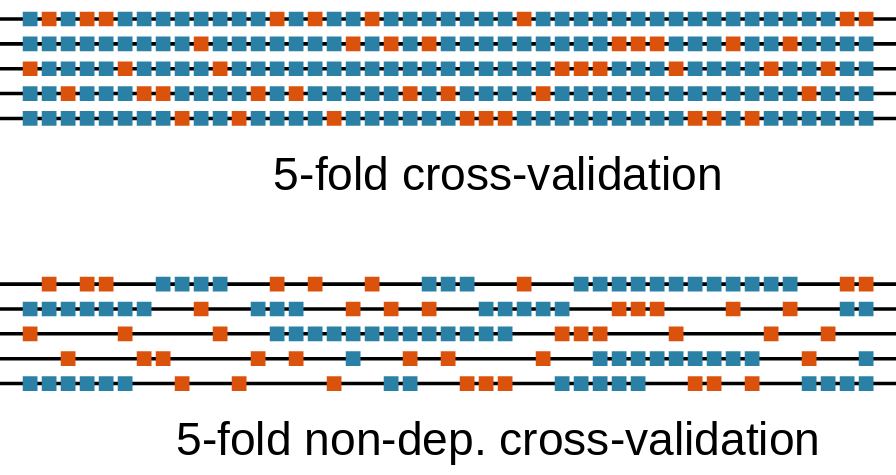
\includegraphics[width=0.9\linewidth]{Imagens/Cross-validation-scheme}
    \caption{$\mathcal{K}$-fold CV and $\mathcal{K}$-fold with non-dependent data. Observations in blue are used to estimation and in orange for evaluation. Note that non-dependent data doesn't use all dataset in each fold.}
    \label{fig:cross-validation-scheme}
\end{figure}

\end{frame}

\begin{frame}{Time-series Cross-Validation}

\begin{itemize}
\tightlist
\item
  The CV score is given by the sum of the loss function for each fold.
  The optimum value of \(t\) in this criteria is the one that minimizes
  the CV score: \[
  \theta^* = \text{argmin}_\theta CV(\theta) = \sum_{k \in \mathcal{K}} \sum_{\alpha \in A} L(\alpha).
  \]
\item
  To optimize CV function in \(\theta\), we use the Nelder-Mead
  algorithm, which is a known and widely used algorithm for black-box
  optimization.
\end{itemize}

\end{frame}

\section{Nonparametric model}\label{nonparametric-model}

\begin{frame}{Nonparametric model - Formulation}

\tiny

\begin{eqnarray}
\min_{q_{\alpha t},\delta^+_{t}, \delta_t^-, \xi_t} & \sum_{\alpha \in A} \sum_{t \in T'}\left(\alpha\delta_{t \alpha }^{+}+(1-\alpha)\delta_{t \alpha }^{-}\right) & \\
& \qquad \qquad \qquad \qquad \qquad + \lambda_1\sum_{t \in T'}\gamma_{t \alpha } + \lambda_2\sum_{t \in T'}\xi_{t \alpha } & \nonumber \\
s.t. & \delta_{t}^{+}-\delta_{t \alpha }^{-}=y_{t}-q_{t \alpha }, & \qquad\forall t \in T',\forall \alpha \in A,\\
   & D^{1}_{t \alpha }=\frac{q_{\alpha t+1}-q_{\alpha t}}{x_{t+1}-x_{t}},
    & \qquad\forall t \in T',\forall \alpha \in A,\\   
 & D^{2}_{t \alpha }=\frac{\left(\frac{q_{\alpha t+1}-q_{\alpha t}}{x_{t+1}-x_{t}}\right)-\left(\frac{q_{\alpha t}-q_{\alpha t-1}}{x_{t}-x_{t-1}}\right)}{x_{t+1}-2x_{t} + x_{t-1}}.
  & \qquad\forall t \in T',\forall \alpha \in A,\\
 & \gamma_{t \alpha}\geq D^1_{t \alpha }, & \qquad\forall t \in T',\forall \alpha \in A,\\
  & \gamma_{t \alpha}\geq-D^1_{t \alpha}, & \qquad\forall t \in T',\forall \alpha \in A,\\
  & \xi_{t \alpha}\geq D^2_{t \alpha }, & \qquad\forall t \in T',\forall \alpha \in A,\\
 & \xi_{t \alpha}\geq-D^2_{t \alpha}, & \qquad\forall t \in T',\forall \alpha \in A,\\
 & \delta_{t \alpha}^{+},\delta_{t \alpha}^{-},\gamma_{t \alpha}, \xi_{t \alpha}\geq0, & \qquad\forall t \in T',\forall \alpha \in A,\\
  & q_{t \alpha} \leq q_{t \alpha'}, & \qquad \forall t \in T', \forall (\alpha, \alpha') \in A \times A, \alpha < \alpha',\nonumber \\  
  \end{eqnarray}

\end{frame}

\begin{frame}{Nonparametric vs.~Linear Model}

\begin{itemize}
\tightlist
\item
  The nonparametric approach is more flexible to capture
  heteroscedasticity.
\end{itemize}

\begin{figure}
  \centering
  \begin{minipage}[t]{\linewidth}
    \centering
    \begin{minipage}[t]{0.45\linewidth}
      \centering     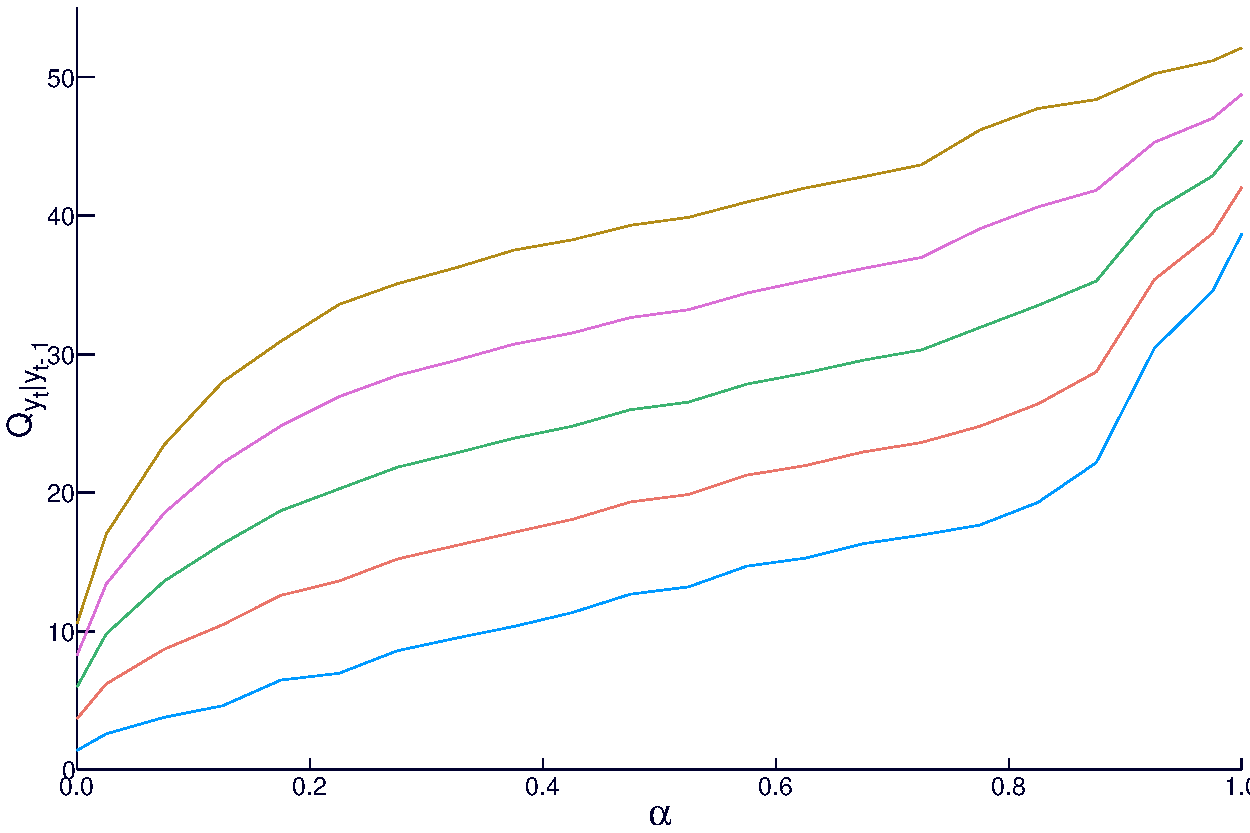
\includegraphics[width=\textwidth]{../Figuras/regressao-quantilica/icaraizinho-quantile-linear}
    \end{minipage}
    \begin{minipage}[t]{0.45\linewidth}
      \centering     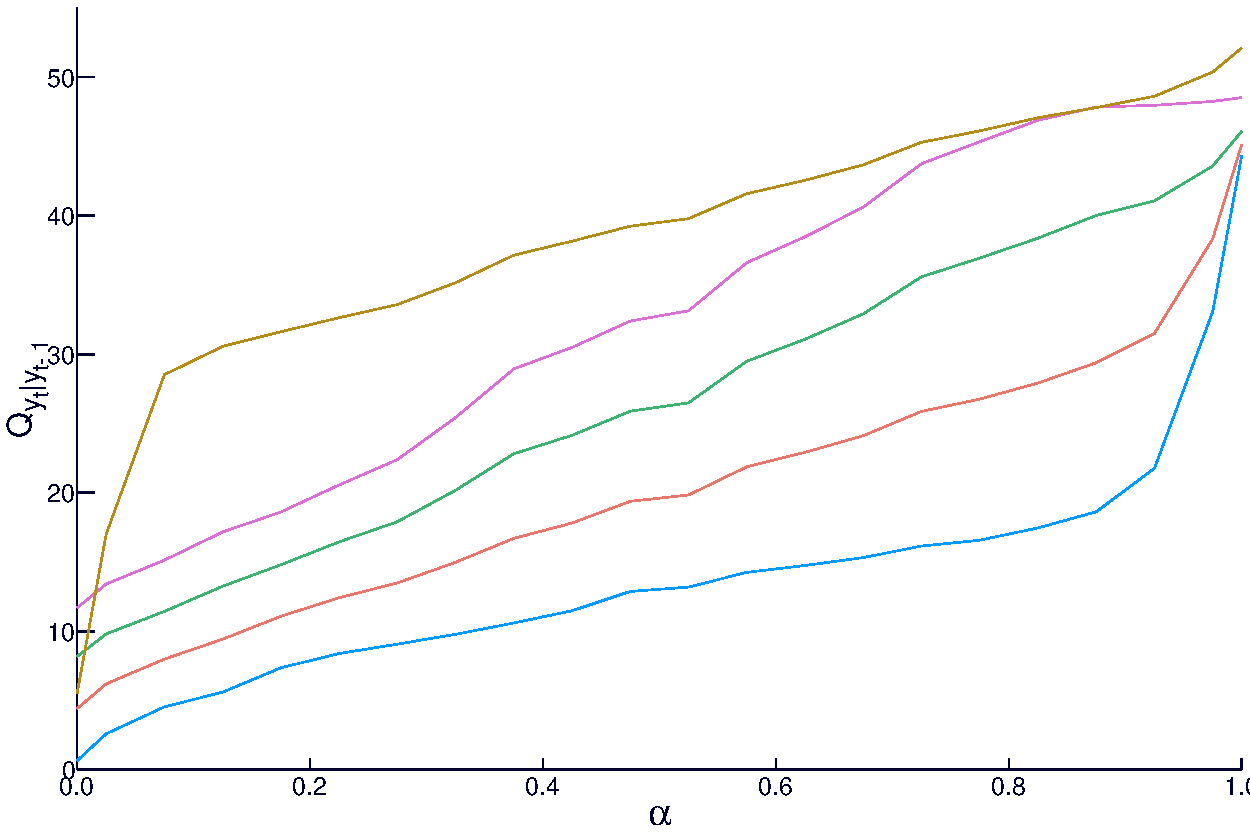
\includegraphics[width=\textwidth]{../Figuras/regressao-quantilica/icaraizinho-quantile-nonpar-lambda30}
    \end{minipage}
  \end{minipage}
  \caption{Estimated quantile functions, for different values of $y_{t-1}$. On the left using a linear model and using a nonparametric approach on the right.}
  \label{fig:quantiles-vs-xt}
\end{figure}

\end{frame}

\begin{frame}{Nonparametric vs.~Linear Model}

\begin{itemize}
\tightlist
\item
  This flexibility might lead to overfitting, if we don't select a
  proper penalty, as shown below:

  \begin{figure}
          \centering     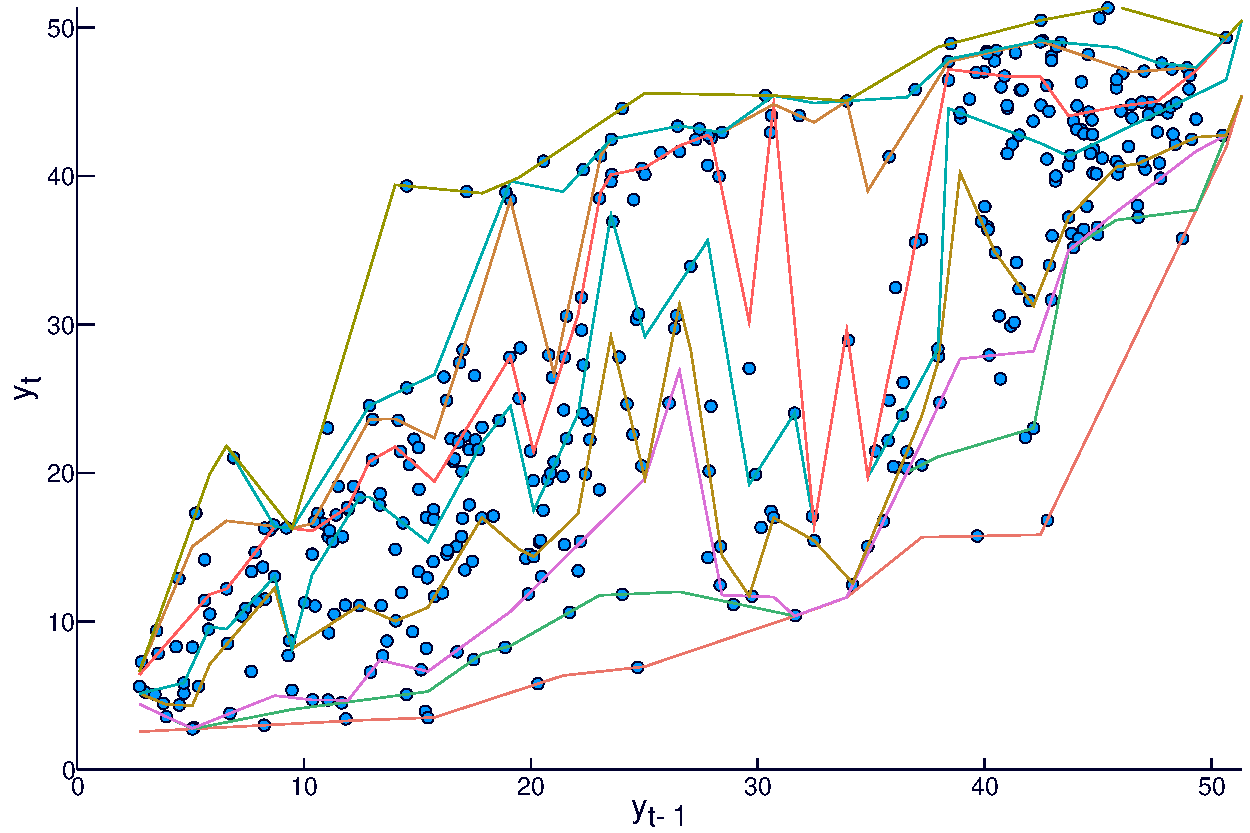
\includegraphics[width=0.6 \textwidth]{../Figuras/regressao-quantilica/icaraizinho-crossing-01}
  \caption{Example of a overfitted quantile function}
  \label{fig:convergence}
  \end{figure}
\end{itemize}

\end{frame}

\section{Final}\label{final}

\begin{frame}{References}

\tiny

\hypertarget{refs}{}
\hypertarget{ref-gallego2016line}{}
Gallego-Castillo, Cristobal, Ricardo Bessa, Laura Cavalcante, and Oscar
Lopez-Garcia. 2016. ``On-Line Quantile Regression in the Rkhs
(Reproducing Kernel Hilbert Space) for Operational Probabilistic
Forecasting of Wind Power.'' \emph{Energy} 113. Elsevier: 355--65.

\hypertarget{ref-koenker1978regression}{}
Koenker, Roger, and Gilbert Bassett Jr. 1978. ``Regression Quantiles.''
\emph{Econometrica: Journal of the Econometric Society}. JSTOR, 33--50.

\hypertarget{ref-wan_direct_2017}{}
Wan, C., J. Lin, J. Wang, Y. Song, and Z. Y. Dong. 2017. ``Direct
Quantile Regression for Nonparametric Probabilistic Forecasting of Wind
Power Generation.'' \emph{IEEE Transactions on Power Systems} 32 (4):
2767--78.
doi:\href{https://doi.org/10.1109/TPWRS.2016.2625101}{10.1109/TPWRS.2016.2625101}.

\end{frame}
